\documentclass[twoside]{book}

% Packages required by doxygen
\usepackage{fixltx2e}
\usepackage{calc}
\usepackage{doxygen}
\usepackage[export]{adjustbox} % also loads graphicx
\usepackage{graphicx}
\usepackage[utf8]{inputenc}
\usepackage{makeidx}
\usepackage{multicol}
\usepackage{multirow}
\PassOptionsToPackage{warn}{textcomp}
\usepackage{textcomp}
\usepackage[nointegrals]{wasysym}
\usepackage[table]{xcolor}

% Font selection
\usepackage[T1]{fontenc}
\usepackage[scaled=.90]{helvet}
\usepackage{courier}
\usepackage{amssymb}
\usepackage{sectsty}
\renewcommand{\familydefault}{\sfdefault}
\allsectionsfont{%
  \fontseries{bc}\selectfont%
  \color{darkgray}%
}
\renewcommand{\DoxyLabelFont}{%
  \fontseries{bc}\selectfont%
  \color{darkgray}%
}
\newcommand{\+}{\discretionary{\mbox{\scriptsize$\hookleftarrow$}}{}{}}

% Page & text layout
\usepackage{geometry}
\geometry{%
  a4paper,%
  top=2.5cm,%
  bottom=2.5cm,%
  left=2.5cm,%
  right=2.5cm%
}
\tolerance=750
\hfuzz=15pt
\hbadness=750
\setlength{\emergencystretch}{15pt}
\setlength{\parindent}{0cm}
\setlength{\parskip}{3ex plus 2ex minus 2ex}
\makeatletter
\renewcommand{\paragraph}{%
  \@startsection{paragraph}{4}{0ex}{-1.0ex}{1.0ex}{%
    \normalfont\normalsize\bfseries\SS@parafont%
  }%
}
\renewcommand{\subparagraph}{%
  \@startsection{subparagraph}{5}{0ex}{-1.0ex}{1.0ex}{%
    \normalfont\normalsize\bfseries\SS@subparafont%
  }%
}
\makeatother

% Headers & footers
\usepackage{fancyhdr}
\pagestyle{fancyplain}
\fancyhead[LE]{\fancyplain{}{\bfseries\thepage}}
\fancyhead[CE]{\fancyplain{}{}}
\fancyhead[RE]{\fancyplain{}{\bfseries\leftmark}}
\fancyhead[LO]{\fancyplain{}{\bfseries\rightmark}}
\fancyhead[CO]{\fancyplain{}{}}
\fancyhead[RO]{\fancyplain{}{\bfseries\thepage}}
\fancyfoot[LE]{\fancyplain{}{}}
\fancyfoot[CE]{\fancyplain{}{}}
\fancyfoot[RE]{\fancyplain{}{\bfseries\scriptsize Generated by Doxygen }}
\fancyfoot[LO]{\fancyplain{}{\bfseries\scriptsize Generated by Doxygen }}
\fancyfoot[CO]{\fancyplain{}{}}
\fancyfoot[RO]{\fancyplain{}{}}
\renewcommand{\footrulewidth}{0.4pt}
\renewcommand{\chaptermark}[1]{%
  \markboth{#1}{}%
}
\renewcommand{\sectionmark}[1]{%
  \markright{\thesection\ #1}%
}

% Indices & bibliography
\usepackage{natbib}
\usepackage[titles]{tocloft}
\setcounter{tocdepth}{3}
\setcounter{secnumdepth}{5}
\makeindex

% Hyperlinks (required, but should be loaded last)
\usepackage{ifpdf}
\ifpdf
  \usepackage[pdftex,pagebackref=true]{hyperref}
\else
  \usepackage[ps2pdf,pagebackref=true]{hyperref}
\fi
\hypersetup{%
  colorlinks=true,%
  linkcolor=blue,%
  citecolor=blue,%
  unicode%
}

% Custom commands
\newcommand{\clearemptydoublepage}{%
  \newpage{\pagestyle{empty}\cleardoublepage}%
}

\usepackage{caption}
\captionsetup{labelsep=space,justification=centering,font={bf},singlelinecheck=off,skip=4pt,position=top}

%===== C O N T E N T S =====

\begin{document}

% Titlepage & ToC
\hypersetup{pageanchor=false,
             bookmarksnumbered=true,
             pdfencoding=unicode
            }
\pagenumbering{alph}
\begin{titlepage}
\vspace*{7cm}
\begin{center}%
{\Large Dualization Artem Tashevtsev }\\
\vspace*{1cm}
{\large Generated by Doxygen 1.8.13}\\
\end{center}
\end{titlepage}
\clearemptydoublepage
\pagenumbering{roman}
\tableofcontents
\clearemptydoublepage
\pagenumbering{arabic}
\hypersetup{pageanchor=true}

%--- Begin generated contents ---
\chapter{Hierarchical Index}
\section{Class Hierarchy}
This inheritance list is sorted roughly, but not completely, alphabetically\+:\begin{DoxyCompactList}
\item \contentsline{section}{Bit\+Matrix}{\pageref{classBitMatrix}}{}
\begin{DoxyCompactList}
\item \contentsline{section}{Partial\+Bit\+Matrix}{\pageref{classPartialBitMatrix}}{}
\end{DoxyCompactList}
\end{DoxyCompactList}

\chapter{Class Index}
\section{Class List}
Here are the classes, structs, unions and interfaces with brief descriptions\+:\begin{DoxyCompactList}
\item\contentsline{section}{\hyperlink{classBitMatrix}{Bit\+Matrix} }{\pageref{classBitMatrix}}{}
\item\contentsline{section}{\hyperlink{classPartialBitMatrix}{Partial\+Bit\+Matrix} }{\pageref{classPartialBitMatrix}}{}
\end{DoxyCompactList}

\chapter{File Index}
\section{File List}
Here is a list of all files with brief descriptions\+:\begin{DoxyCompactList}
\item\contentsline{section}{\hyperlink{main_8cpp}{main.\+cpp} }{\pageref{main_8cpp}}{}
\end{DoxyCompactList}

\chapter{Class Documentation}
\hypertarget{classBitMatrix}{}\section{Bit\+Matrix Class Reference}
\label{classBitMatrix}\index{Bit\+Matrix@{Bit\+Matrix}}


Inheritance diagram for Bit\+Matrix\+:
\nopagebreak
\begin{figure}[H]
\begin{center}
\leavevmode
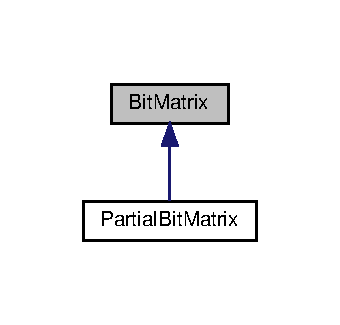
\includegraphics[width=163pt]{classBitMatrix__inherit__graph}
\end{center}
\end{figure}
\subsection*{Public Member Functions}
\begin{DoxyCompactItemize}
\item 
\hyperlink{classBitMatrix_aea3afaf70111c302f23971bbb84dee10}{Bit\+Matrix} (istream \&in, size\+\_\+t n, size\+\_\+t m)
\item 
\hyperlink{classBitMatrix_a47e8b65693dc2e86541d0098232654a7}{Bit\+Matrix} (const string \&filename, size\+\_\+t n, size\+\_\+t m)
\item 
\hyperlink{classBitMatrix_aa264bc0bfe4a54ca8e0cafcd17aaddd1}{$\sim$\+Bit\+Matrix} ()
\item 
size\+\_\+t \hyperlink{classBitMatrix_a45b01a2a1e0cd1227cbe06d0c47c35d1}{get\+Height} () const
\item 
size\+\_\+t \hyperlink{classBitMatrix_ae4bf5529a6676a836a0ff965285e9907}{get\+Width} () const
\item 
size\+\_\+t \hyperlink{classBitMatrix_ac4ddfe5f94dba2904d9d6319bbdd8012}{get\+Chunks} () const
\item 
const vector$<$ vector$<$ \hyperlink{main_8cpp_a49d1cb44c18ad3e6cc52845f905e6181}{ull} $>$ $>$ \& \hyperlink{classBitMatrix_a167706d1d6576f29382fc55b5c99884d}{get\+Matrix} () const
\item 
int \hyperlink{classBitMatrix_a4ec563a3bf6d62141d719ebeed5348e8}{at} (size\+\_\+t i, size\+\_\+t j) const
\end{DoxyCompactItemize}
\subsection*{Private Attributes}
\begin{DoxyCompactItemize}
\item 
vector$<$ vector$<$ \hyperlink{main_8cpp_a49d1cb44c18ad3e6cc52845f905e6181}{ull} $>$ $>$ \hyperlink{classBitMatrix_abe5132a2524a8c5d5e5a11d0f4753bc6}{matrix}
\item 
size\+\_\+t \hyperlink{classBitMatrix_a546978092da7a641ac9c23daa88a31ae}{height}
\item 
size\+\_\+t \hyperlink{classBitMatrix_a8f75a335960dd7af6fc791f43bc3a8c1}{width}
\item 
size\+\_\+t \hyperlink{classBitMatrix_af4a0d4517ff5a485c5787150f9e6a545}{chunks}
\end{DoxyCompactItemize}
\subsection*{Friends}
\begin{DoxyCompactItemize}
\item 
ostream \& \hyperlink{classBitMatrix_aa35d89b587731633f4de5309b083689b}{operator$<$$<$} (ostream \&os, const \hyperlink{classBitMatrix}{Bit\+Matrix} \&bm)
\end{DoxyCompactItemize}


\subsection{Detailed Description}
A simple class for binary matrix stored as bit sets 

\subsection{Constructor \& Destructor Documentation}
\mbox{\Hypertarget{classBitMatrix_aea3afaf70111c302f23971bbb84dee10}\label{classBitMatrix_aea3afaf70111c302f23971bbb84dee10}} 
\index{Bit\+Matrix@{Bit\+Matrix}!Bit\+Matrix@{Bit\+Matrix}}
\index{Bit\+Matrix@{Bit\+Matrix}!Bit\+Matrix@{Bit\+Matrix}}
\subsubsection{\texorpdfstring{Bit\+Matrix()}{BitMatrix()}\hspace{0.1cm}{\footnotesize\ttfamily [1/2]}}
{\footnotesize\ttfamily Bit\+Matrix\+::\+Bit\+Matrix (\begin{DoxyParamCaption}\item[{istream \&}]{in,  }\item[{size\+\_\+t}]{n,  }\item[{size\+\_\+t}]{m }\end{DoxyParamCaption})\hspace{0.3cm}{\ttfamily [inline]}}

\mbox{\Hypertarget{classBitMatrix_a47e8b65693dc2e86541d0098232654a7}\label{classBitMatrix_a47e8b65693dc2e86541d0098232654a7}} 
\index{Bit\+Matrix@{Bit\+Matrix}!Bit\+Matrix@{Bit\+Matrix}}
\index{Bit\+Matrix@{Bit\+Matrix}!Bit\+Matrix@{Bit\+Matrix}}
\subsubsection{\texorpdfstring{Bit\+Matrix()}{BitMatrix()}\hspace{0.1cm}{\footnotesize\ttfamily [2/2]}}
{\footnotesize\ttfamily Bit\+Matrix\+::\+Bit\+Matrix (\begin{DoxyParamCaption}\item[{const string \&}]{filename,  }\item[{size\+\_\+t}]{n,  }\item[{size\+\_\+t}]{m }\end{DoxyParamCaption})\hspace{0.3cm}{\ttfamily [inline]}}

\mbox{\Hypertarget{classBitMatrix_aa264bc0bfe4a54ca8e0cafcd17aaddd1}\label{classBitMatrix_aa264bc0bfe4a54ca8e0cafcd17aaddd1}} 
\index{Bit\+Matrix@{Bit\+Matrix}!````~Bit\+Matrix@{$\sim$\+Bit\+Matrix}}
\index{````~Bit\+Matrix@{$\sim$\+Bit\+Matrix}!Bit\+Matrix@{Bit\+Matrix}}
\subsubsection{\texorpdfstring{$\sim$\+Bit\+Matrix()}{~BitMatrix()}}
{\footnotesize\ttfamily Bit\+Matrix\+::$\sim$\+Bit\+Matrix (\begin{DoxyParamCaption}{ }\end{DoxyParamCaption})\hspace{0.3cm}{\ttfamily [inline]}}



\subsection{Member Function Documentation}
\mbox{\Hypertarget{classBitMatrix_a4ec563a3bf6d62141d719ebeed5348e8}\label{classBitMatrix_a4ec563a3bf6d62141d719ebeed5348e8}} 
\index{Bit\+Matrix@{Bit\+Matrix}!at@{at}}
\index{at@{at}!Bit\+Matrix@{Bit\+Matrix}}
\subsubsection{\texorpdfstring{at()}{at()}}
{\footnotesize\ttfamily int Bit\+Matrix\+::at (\begin{DoxyParamCaption}\item[{size\+\_\+t}]{i,  }\item[{size\+\_\+t}]{j }\end{DoxyParamCaption}) const\hspace{0.3cm}{\ttfamily [inline]}}

\mbox{\Hypertarget{classBitMatrix_ac4ddfe5f94dba2904d9d6319bbdd8012}\label{classBitMatrix_ac4ddfe5f94dba2904d9d6319bbdd8012}} 
\index{Bit\+Matrix@{Bit\+Matrix}!get\+Chunks@{get\+Chunks}}
\index{get\+Chunks@{get\+Chunks}!Bit\+Matrix@{Bit\+Matrix}}
\subsubsection{\texorpdfstring{get\+Chunks()}{getChunks()}}
{\footnotesize\ttfamily size\+\_\+t Bit\+Matrix\+::get\+Chunks (\begin{DoxyParamCaption}{ }\end{DoxyParamCaption}) const\hspace{0.3cm}{\ttfamily [inline]}}

\mbox{\Hypertarget{classBitMatrix_a45b01a2a1e0cd1227cbe06d0c47c35d1}\label{classBitMatrix_a45b01a2a1e0cd1227cbe06d0c47c35d1}} 
\index{Bit\+Matrix@{Bit\+Matrix}!get\+Height@{get\+Height}}
\index{get\+Height@{get\+Height}!Bit\+Matrix@{Bit\+Matrix}}
\subsubsection{\texorpdfstring{get\+Height()}{getHeight()}}
{\footnotesize\ttfamily size\+\_\+t Bit\+Matrix\+::get\+Height (\begin{DoxyParamCaption}{ }\end{DoxyParamCaption}) const\hspace{0.3cm}{\ttfamily [inline]}}

\mbox{\Hypertarget{classBitMatrix_a167706d1d6576f29382fc55b5c99884d}\label{classBitMatrix_a167706d1d6576f29382fc55b5c99884d}} 
\index{Bit\+Matrix@{Bit\+Matrix}!get\+Matrix@{get\+Matrix}}
\index{get\+Matrix@{get\+Matrix}!Bit\+Matrix@{Bit\+Matrix}}
\subsubsection{\texorpdfstring{get\+Matrix()}{getMatrix()}}
{\footnotesize\ttfamily const vector$<$vector$<$\hyperlink{main_8cpp_a49d1cb44c18ad3e6cc52845f905e6181}{ull}$>$ $>$\& Bit\+Matrix\+::get\+Matrix (\begin{DoxyParamCaption}{ }\end{DoxyParamCaption}) const\hspace{0.3cm}{\ttfamily [inline]}}

\mbox{\Hypertarget{classBitMatrix_ae4bf5529a6676a836a0ff965285e9907}\label{classBitMatrix_ae4bf5529a6676a836a0ff965285e9907}} 
\index{Bit\+Matrix@{Bit\+Matrix}!get\+Width@{get\+Width}}
\index{get\+Width@{get\+Width}!Bit\+Matrix@{Bit\+Matrix}}
\subsubsection{\texorpdfstring{get\+Width()}{getWidth()}}
{\footnotesize\ttfamily size\+\_\+t Bit\+Matrix\+::get\+Width (\begin{DoxyParamCaption}{ }\end{DoxyParamCaption}) const\hspace{0.3cm}{\ttfamily [inline]}}



\subsection{Friends And Related Function Documentation}
\mbox{\Hypertarget{classBitMatrix_aa35d89b587731633f4de5309b083689b}\label{classBitMatrix_aa35d89b587731633f4de5309b083689b}} 
\index{Bit\+Matrix@{Bit\+Matrix}!operator$<$$<$@{operator$<$$<$}}
\index{operator$<$$<$@{operator$<$$<$}!Bit\+Matrix@{Bit\+Matrix}}
\subsubsection{\texorpdfstring{operator$<$$<$}{operator<<}}
{\footnotesize\ttfamily ostream\& operator$<$$<$ (\begin{DoxyParamCaption}\item[{ostream \&}]{os,  }\item[{const \hyperlink{classBitMatrix}{Bit\+Matrix} \&}]{bm }\end{DoxyParamCaption})\hspace{0.3cm}{\ttfamily [friend]}}



\subsection{Member Data Documentation}
\mbox{\Hypertarget{classBitMatrix_af4a0d4517ff5a485c5787150f9e6a545}\label{classBitMatrix_af4a0d4517ff5a485c5787150f9e6a545}} 
\index{Bit\+Matrix@{Bit\+Matrix}!chunks@{chunks}}
\index{chunks@{chunks}!Bit\+Matrix@{Bit\+Matrix}}
\subsubsection{\texorpdfstring{chunks}{chunks}}
{\footnotesize\ttfamily size\+\_\+t Bit\+Matrix\+::chunks\hspace{0.3cm}{\ttfamily [private]}}

\mbox{\Hypertarget{classBitMatrix_a546978092da7a641ac9c23daa88a31ae}\label{classBitMatrix_a546978092da7a641ac9c23daa88a31ae}} 
\index{Bit\+Matrix@{Bit\+Matrix}!height@{height}}
\index{height@{height}!Bit\+Matrix@{Bit\+Matrix}}
\subsubsection{\texorpdfstring{height}{height}}
{\footnotesize\ttfamily size\+\_\+t Bit\+Matrix\+::height\hspace{0.3cm}{\ttfamily [private]}}

\mbox{\Hypertarget{classBitMatrix_abe5132a2524a8c5d5e5a11d0f4753bc6}\label{classBitMatrix_abe5132a2524a8c5d5e5a11d0f4753bc6}} 
\index{Bit\+Matrix@{Bit\+Matrix}!matrix@{matrix}}
\index{matrix@{matrix}!Bit\+Matrix@{Bit\+Matrix}}
\subsubsection{\texorpdfstring{matrix}{matrix}}
{\footnotesize\ttfamily vector$<$vector$<$\hyperlink{main_8cpp_a49d1cb44c18ad3e6cc52845f905e6181}{ull}$>$ $>$ Bit\+Matrix\+::matrix\hspace{0.3cm}{\ttfamily [private]}}

The matrix where all data is stored \mbox{\Hypertarget{classBitMatrix_a8f75a335960dd7af6fc791f43bc3a8c1}\label{classBitMatrix_a8f75a335960dd7af6fc791f43bc3a8c1}} 
\index{Bit\+Matrix@{Bit\+Matrix}!width@{width}}
\index{width@{width}!Bit\+Matrix@{Bit\+Matrix}}
\subsubsection{\texorpdfstring{width}{width}}
{\footnotesize\ttfamily size\+\_\+t Bit\+Matrix\+::width\hspace{0.3cm}{\ttfamily [private]}}



The documentation for this class was generated from the following file\+:\begin{DoxyCompactItemize}
\item 
\hyperlink{main_8cpp}{main.\+cpp}\end{DoxyCompactItemize}

\hypertarget{classPartialBitMatrix}{}\section{Partial\+Bit\+Matrix Class Reference}
\label{classPartialBitMatrix}\index{Partial\+Bit\+Matrix@{Partial\+Bit\+Matrix}}


Inheritance diagram for Partial\+Bit\+Matrix\+:
\nopagebreak
\begin{figure}[H]
\begin{center}
\leavevmode
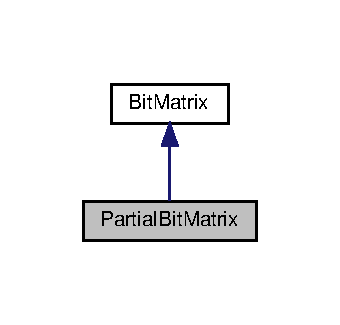
\includegraphics[width=163pt]{classPartialBitMatrix__inherit__graph}
\end{center}
\end{figure}


Collaboration diagram for Partial\+Bit\+Matrix\+:
\nopagebreak
\begin{figure}[H]
\begin{center}
\leavevmode
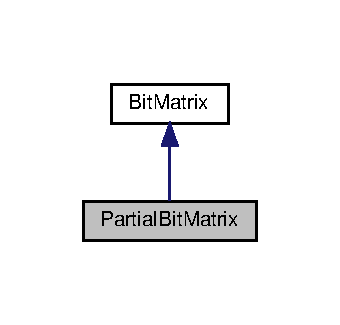
\includegraphics[width=163pt]{classPartialBitMatrix__coll__graph}
\end{center}
\end{figure}
\subsection*{Public Member Functions}
\begin{DoxyCompactItemize}
\item 
\hyperlink{classPartialBitMatrix_a0bdc388b54ece3f0af522140f1d8fa3f}{Partial\+Bit\+Matrix} (istream \&in, size\+\_\+t n, size\+\_\+t m)
\item 
\hyperlink{classPartialBitMatrix_a9c57752eb3d83c96694d6016ab51b93f}{Partial\+Bit\+Matrix} (const string \&filename, size\+\_\+t n, size\+\_\+t m)
\item 
bool \hyperlink{classPartialBitMatrix_a14711125645f4395fbf834ba10e7e538}{delete\+\_\+column} (size\+\_\+t col)
\item 
bool \hyperlink{classPartialBitMatrix_a29612f1d11f0e53c889b23ec9db445ba}{delete\+\_\+row} (size\+\_\+t row)
\item 
size\+\_\+t \hyperlink{classPartialBitMatrix_ac6e4c5182f8c04323cd2fde465021756}{get\+Cur\+\_\+height} () const
\item 
size\+\_\+t \hyperlink{classPartialBitMatrix_a9bd1557769214ae8442b57c561015a96}{get\+Cur\+\_\+width} () const
\item 
const set$<$ size\+\_\+t $>$ \& \hyperlink{classPartialBitMatrix_ab3ffe36bd4034cb0b28f53064bde5309}{get\+Available\+\_\+rows} () const
\item 
const set$<$ size\+\_\+t $>$ \& \hyperlink{classPartialBitMatrix_ab6d7d19a7c87ec6c397b336121f37712}{get\+Available\+\_\+cols} () const
\end{DoxyCompactItemize}
\subsection*{Private Member Functions}
\begin{DoxyCompactItemize}
\item 
void \hyperlink{classPartialBitMatrix_ab0e8e1dc7a71ab0b9203fd13bc748c0f}{delete\+\_\+zero\+\_\+columns} ()
\item 
void \hyperlink{classPartialBitMatrix_a9e08f3b006f85bcec3853a1df320decd}{delete\+\_\+wider\+\_\+rows} ()
\end{DoxyCompactItemize}
\subsection*{Private Attributes}
\begin{DoxyCompactItemize}
\item 
set$<$ size\+\_\+t $>$ \hyperlink{classPartialBitMatrix_a424c7cd6f2af62cf9356e53a7898c051}{available\+\_\+rows}
\item 
set$<$ size\+\_\+t $>$ \hyperlink{classPartialBitMatrix_a1c44d05b37ba0acb4fbf05ae39d44de3}{available\+\_\+cols}
\item 
size\+\_\+t \hyperlink{classPartialBitMatrix_ad6f7fd9eb7ecd63d44419c8388cdebf1}{cur\+\_\+height}
\item 
size\+\_\+t \hyperlink{classPartialBitMatrix_a5684506338c5c27b8936f42e34107267}{cur\+\_\+width}
\end{DoxyCompactItemize}
\subsection*{Friends}
\begin{DoxyCompactItemize}
\item 
ostream \& \hyperlink{classPartialBitMatrix_ad47fa6477b5477654c809695f108d52e}{operator$<$$<$} (ostream \&os, const \hyperlink{classPartialBitMatrix}{Partial\+Bit\+Matrix} \&bm)
\end{DoxyCompactItemize}


\subsection{Constructor \& Destructor Documentation}
\mbox{\Hypertarget{classPartialBitMatrix_a0bdc388b54ece3f0af522140f1d8fa3f}\label{classPartialBitMatrix_a0bdc388b54ece3f0af522140f1d8fa3f}} 
\index{Partial\+Bit\+Matrix@{Partial\+Bit\+Matrix}!Partial\+Bit\+Matrix@{Partial\+Bit\+Matrix}}
\index{Partial\+Bit\+Matrix@{Partial\+Bit\+Matrix}!Partial\+Bit\+Matrix@{Partial\+Bit\+Matrix}}
\subsubsection{\texorpdfstring{Partial\+Bit\+Matrix()}{PartialBitMatrix()}\hspace{0.1cm}{\footnotesize\ttfamily [1/2]}}
{\footnotesize\ttfamily Partial\+Bit\+Matrix\+::\+Partial\+Bit\+Matrix (\begin{DoxyParamCaption}\item[{istream \&}]{in,  }\item[{size\+\_\+t}]{n,  }\item[{size\+\_\+t}]{m }\end{DoxyParamCaption})\hspace{0.3cm}{\ttfamily [inline]}}

\mbox{\Hypertarget{classPartialBitMatrix_a9c57752eb3d83c96694d6016ab51b93f}\label{classPartialBitMatrix_a9c57752eb3d83c96694d6016ab51b93f}} 
\index{Partial\+Bit\+Matrix@{Partial\+Bit\+Matrix}!Partial\+Bit\+Matrix@{Partial\+Bit\+Matrix}}
\index{Partial\+Bit\+Matrix@{Partial\+Bit\+Matrix}!Partial\+Bit\+Matrix@{Partial\+Bit\+Matrix}}
\subsubsection{\texorpdfstring{Partial\+Bit\+Matrix()}{PartialBitMatrix()}\hspace{0.1cm}{\footnotesize\ttfamily [2/2]}}
{\footnotesize\ttfamily Partial\+Bit\+Matrix\+::\+Partial\+Bit\+Matrix (\begin{DoxyParamCaption}\item[{const string \&}]{filename,  }\item[{size\+\_\+t}]{n,  }\item[{size\+\_\+t}]{m }\end{DoxyParamCaption})\hspace{0.3cm}{\ttfamily [inline]}}



\subsection{Member Function Documentation}
\mbox{\Hypertarget{classPartialBitMatrix_a14711125645f4395fbf834ba10e7e538}\label{classPartialBitMatrix_a14711125645f4395fbf834ba10e7e538}} 
\index{Partial\+Bit\+Matrix@{Partial\+Bit\+Matrix}!delete\+\_\+column@{delete\+\_\+column}}
\index{delete\+\_\+column@{delete\+\_\+column}!Partial\+Bit\+Matrix@{Partial\+Bit\+Matrix}}
\subsubsection{\texorpdfstring{delete\+\_\+column()}{delete\_column()}}
{\footnotesize\ttfamily bool Partial\+Bit\+Matrix\+::delete\+\_\+column (\begin{DoxyParamCaption}\item[{size\+\_\+t}]{col }\end{DoxyParamCaption})\hspace{0.3cm}{\ttfamily [inline]}}

\mbox{\Hypertarget{classPartialBitMatrix_a29612f1d11f0e53c889b23ec9db445ba}\label{classPartialBitMatrix_a29612f1d11f0e53c889b23ec9db445ba}} 
\index{Partial\+Bit\+Matrix@{Partial\+Bit\+Matrix}!delete\+\_\+row@{delete\+\_\+row}}
\index{delete\+\_\+row@{delete\+\_\+row}!Partial\+Bit\+Matrix@{Partial\+Bit\+Matrix}}
\subsubsection{\texorpdfstring{delete\+\_\+row()}{delete\_row()}}
{\footnotesize\ttfamily bool Partial\+Bit\+Matrix\+::delete\+\_\+row (\begin{DoxyParamCaption}\item[{size\+\_\+t}]{row }\end{DoxyParamCaption})\hspace{0.3cm}{\ttfamily [inline]}}


\begin{DoxyParams}{Parameters}
{\em row} & \\
\hline
\end{DoxyParams}
\begin{DoxyReturn}{Returns}

\end{DoxyReturn}
\mbox{\Hypertarget{classPartialBitMatrix_a9e08f3b006f85bcec3853a1df320decd}\label{classPartialBitMatrix_a9e08f3b006f85bcec3853a1df320decd}} 
\index{Partial\+Bit\+Matrix@{Partial\+Bit\+Matrix}!delete\+\_\+wider\+\_\+rows@{delete\+\_\+wider\+\_\+rows}}
\index{delete\+\_\+wider\+\_\+rows@{delete\+\_\+wider\+\_\+rows}!Partial\+Bit\+Matrix@{Partial\+Bit\+Matrix}}
\subsubsection{\texorpdfstring{delete\+\_\+wider\+\_\+rows()}{delete\_wider\_rows()}}
{\footnotesize\ttfamily void Partial\+Bit\+Matrix\+::delete\+\_\+wider\+\_\+rows (\begin{DoxyParamCaption}{ }\end{DoxyParamCaption})\hspace{0.3cm}{\ttfamily [inline]}, {\ttfamily [private]}}

\mbox{\Hypertarget{classPartialBitMatrix_ab0e8e1dc7a71ab0b9203fd13bc748c0f}\label{classPartialBitMatrix_ab0e8e1dc7a71ab0b9203fd13bc748c0f}} 
\index{Partial\+Bit\+Matrix@{Partial\+Bit\+Matrix}!delete\+\_\+zero\+\_\+columns@{delete\+\_\+zero\+\_\+columns}}
\index{delete\+\_\+zero\+\_\+columns@{delete\+\_\+zero\+\_\+columns}!Partial\+Bit\+Matrix@{Partial\+Bit\+Matrix}}
\subsubsection{\texorpdfstring{delete\+\_\+zero\+\_\+columns()}{delete\_zero\_columns()}}
{\footnotesize\ttfamily void Partial\+Bit\+Matrix\+::delete\+\_\+zero\+\_\+columns (\begin{DoxyParamCaption}{ }\end{DoxyParamCaption})\hspace{0.3cm}{\ttfamily [inline]}, {\ttfamily [private]}}

\mbox{\Hypertarget{classPartialBitMatrix_ab6d7d19a7c87ec6c397b336121f37712}\label{classPartialBitMatrix_ab6d7d19a7c87ec6c397b336121f37712}} 
\index{Partial\+Bit\+Matrix@{Partial\+Bit\+Matrix}!get\+Available\+\_\+cols@{get\+Available\+\_\+cols}}
\index{get\+Available\+\_\+cols@{get\+Available\+\_\+cols}!Partial\+Bit\+Matrix@{Partial\+Bit\+Matrix}}
\subsubsection{\texorpdfstring{get\+Available\+\_\+cols()}{getAvailable\_cols()}}
{\footnotesize\ttfamily const set$<$size\+\_\+t$>$\& Partial\+Bit\+Matrix\+::get\+Available\+\_\+cols (\begin{DoxyParamCaption}{ }\end{DoxyParamCaption}) const\hspace{0.3cm}{\ttfamily [inline]}}

\mbox{\Hypertarget{classPartialBitMatrix_ab3ffe36bd4034cb0b28f53064bde5309}\label{classPartialBitMatrix_ab3ffe36bd4034cb0b28f53064bde5309}} 
\index{Partial\+Bit\+Matrix@{Partial\+Bit\+Matrix}!get\+Available\+\_\+rows@{get\+Available\+\_\+rows}}
\index{get\+Available\+\_\+rows@{get\+Available\+\_\+rows}!Partial\+Bit\+Matrix@{Partial\+Bit\+Matrix}}
\subsubsection{\texorpdfstring{get\+Available\+\_\+rows()}{getAvailable\_rows()}}
{\footnotesize\ttfamily const set$<$size\+\_\+t$>$\& Partial\+Bit\+Matrix\+::get\+Available\+\_\+rows (\begin{DoxyParamCaption}{ }\end{DoxyParamCaption}) const\hspace{0.3cm}{\ttfamily [inline]}}

\mbox{\Hypertarget{classPartialBitMatrix_ac6e4c5182f8c04323cd2fde465021756}\label{classPartialBitMatrix_ac6e4c5182f8c04323cd2fde465021756}} 
\index{Partial\+Bit\+Matrix@{Partial\+Bit\+Matrix}!get\+Cur\+\_\+height@{get\+Cur\+\_\+height}}
\index{get\+Cur\+\_\+height@{get\+Cur\+\_\+height}!Partial\+Bit\+Matrix@{Partial\+Bit\+Matrix}}
\subsubsection{\texorpdfstring{get\+Cur\+\_\+height()}{getCur\_height()}}
{\footnotesize\ttfamily size\+\_\+t Partial\+Bit\+Matrix\+::get\+Cur\+\_\+height (\begin{DoxyParamCaption}{ }\end{DoxyParamCaption}) const\hspace{0.3cm}{\ttfamily [inline]}}

\mbox{\Hypertarget{classPartialBitMatrix_a9bd1557769214ae8442b57c561015a96}\label{classPartialBitMatrix_a9bd1557769214ae8442b57c561015a96}} 
\index{Partial\+Bit\+Matrix@{Partial\+Bit\+Matrix}!get\+Cur\+\_\+width@{get\+Cur\+\_\+width}}
\index{get\+Cur\+\_\+width@{get\+Cur\+\_\+width}!Partial\+Bit\+Matrix@{Partial\+Bit\+Matrix}}
\subsubsection{\texorpdfstring{get\+Cur\+\_\+width()}{getCur\_width()}}
{\footnotesize\ttfamily size\+\_\+t Partial\+Bit\+Matrix\+::get\+Cur\+\_\+width (\begin{DoxyParamCaption}{ }\end{DoxyParamCaption}) const\hspace{0.3cm}{\ttfamily [inline]}}



\subsection{Friends And Related Function Documentation}
\mbox{\Hypertarget{classPartialBitMatrix_ad47fa6477b5477654c809695f108d52e}\label{classPartialBitMatrix_ad47fa6477b5477654c809695f108d52e}} 
\index{Partial\+Bit\+Matrix@{Partial\+Bit\+Matrix}!operator$<$$<$@{operator$<$$<$}}
\index{operator$<$$<$@{operator$<$$<$}!Partial\+Bit\+Matrix@{Partial\+Bit\+Matrix}}
\subsubsection{\texorpdfstring{operator$<$$<$}{operator<<}}
{\footnotesize\ttfamily ostream\& operator$<$$<$ (\begin{DoxyParamCaption}\item[{ostream \&}]{os,  }\item[{const \hyperlink{classPartialBitMatrix}{Partial\+Bit\+Matrix} \&}]{bm }\end{DoxyParamCaption})\hspace{0.3cm}{\ttfamily [friend]}}



\subsection{Member Data Documentation}
\mbox{\Hypertarget{classPartialBitMatrix_a1c44d05b37ba0acb4fbf05ae39d44de3}\label{classPartialBitMatrix_a1c44d05b37ba0acb4fbf05ae39d44de3}} 
\index{Partial\+Bit\+Matrix@{Partial\+Bit\+Matrix}!available\+\_\+cols@{available\+\_\+cols}}
\index{available\+\_\+cols@{available\+\_\+cols}!Partial\+Bit\+Matrix@{Partial\+Bit\+Matrix}}
\subsubsection{\texorpdfstring{available\+\_\+cols}{available\_cols}}
{\footnotesize\ttfamily set$<$size\+\_\+t$>$ Partial\+Bit\+Matrix\+::available\+\_\+cols\hspace{0.3cm}{\ttfamily [private]}}

\mbox{\Hypertarget{classPartialBitMatrix_a424c7cd6f2af62cf9356e53a7898c051}\label{classPartialBitMatrix_a424c7cd6f2af62cf9356e53a7898c051}} 
\index{Partial\+Bit\+Matrix@{Partial\+Bit\+Matrix}!available\+\_\+rows@{available\+\_\+rows}}
\index{available\+\_\+rows@{available\+\_\+rows}!Partial\+Bit\+Matrix@{Partial\+Bit\+Matrix}}
\subsubsection{\texorpdfstring{available\+\_\+rows}{available\_rows}}
{\footnotesize\ttfamily set$<$size\+\_\+t$>$ Partial\+Bit\+Matrix\+::available\+\_\+rows\hspace{0.3cm}{\ttfamily [private]}}

\mbox{\Hypertarget{classPartialBitMatrix_ad6f7fd9eb7ecd63d44419c8388cdebf1}\label{classPartialBitMatrix_ad6f7fd9eb7ecd63d44419c8388cdebf1}} 
\index{Partial\+Bit\+Matrix@{Partial\+Bit\+Matrix}!cur\+\_\+height@{cur\+\_\+height}}
\index{cur\+\_\+height@{cur\+\_\+height}!Partial\+Bit\+Matrix@{Partial\+Bit\+Matrix}}
\subsubsection{\texorpdfstring{cur\+\_\+height}{cur\_height}}
{\footnotesize\ttfamily size\+\_\+t Partial\+Bit\+Matrix\+::cur\+\_\+height\hspace{0.3cm}{\ttfamily [private]}}

\mbox{\Hypertarget{classPartialBitMatrix_a5684506338c5c27b8936f42e34107267}\label{classPartialBitMatrix_a5684506338c5c27b8936f42e34107267}} 
\index{Partial\+Bit\+Matrix@{Partial\+Bit\+Matrix}!cur\+\_\+width@{cur\+\_\+width}}
\index{cur\+\_\+width@{cur\+\_\+width}!Partial\+Bit\+Matrix@{Partial\+Bit\+Matrix}}
\subsubsection{\texorpdfstring{cur\+\_\+width}{cur\_width}}
{\footnotesize\ttfamily size\+\_\+t Partial\+Bit\+Matrix\+::cur\+\_\+width\hspace{0.3cm}{\ttfamily [private]}}



The documentation for this class was generated from the following file\+:\begin{DoxyCompactItemize}
\item 
\hyperlink{main_8cpp}{main.\+cpp}\end{DoxyCompactItemize}

\chapter{File Documentation}
\hypertarget{main_8cpp}{}\section{main.\+cpp File Reference}
\label{main_8cpp}\index{main.\+cpp@{main.\+cpp}}
{\ttfamily \#include $<$iostream$>$}\newline
{\ttfamily \#include $<$vector$>$}\newline
{\ttfamily \#include $<$map$>$}\newline
{\ttfamily \#include $<$set$>$}\newline
{\ttfamily \#include $<$string$>$}\newline
{\ttfamily \#include $<$random$>$}\newline
{\ttfamily \#include $<$fstream$>$}\newline
{\ttfamily \#include $<$cerrno$>$}\newline
{\ttfamily \#include $<$cstring$>$}\newline
Include dependency graph for main.\+cpp\+:
\nopagebreak
\begin{figure}[H]
\begin{center}
\leavevmode
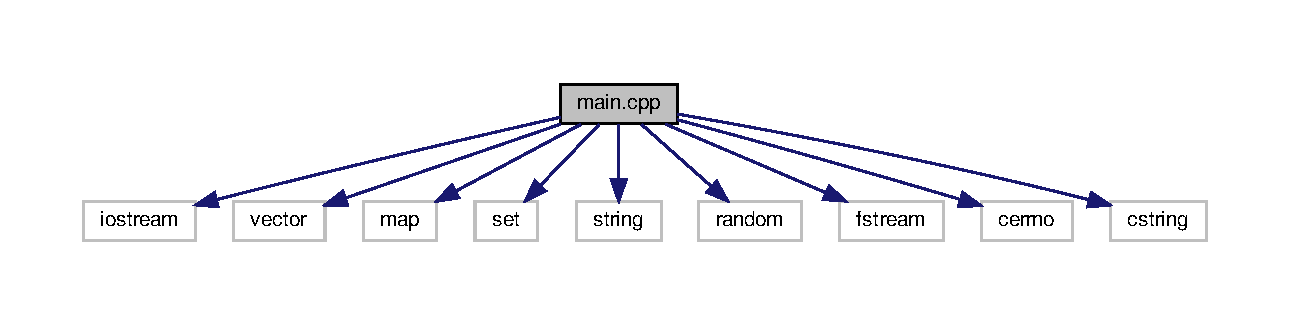
\includegraphics[width=350pt]{main_8cpp__incl}
\end{center}
\end{figure}
\subsection*{Classes}
\begin{DoxyCompactItemize}
\item 
class \hyperlink{classBitMatrix}{Bit\+Matrix}
\item 
class \hyperlink{classPartialBitMatrix}{Partial\+Bit\+Matrix}
\end{DoxyCompactItemize}
\subsection*{Typedefs}
\begin{DoxyCompactItemize}
\item 
typedef uint64\+\_\+t \hyperlink{main_8cpp_a49d1cb44c18ad3e6cc52845f905e6181}{ull}
\end{DoxyCompactItemize}
\subsection*{Enumerations}
\begin{DoxyCompactItemize}
\item 
enum \{ \hyperlink{main_8cpp_a06fc87d81c62e9abb8790b6e5713c55ba14dadc12171e56bbc5360222ea206ff4}{C\+H\+U\+N\+K\+\_\+\+S\+I\+ZE} = sizeof(ull)
 \}
\end{DoxyCompactItemize}
\subsection*{Functions}
\begin{DoxyCompactItemize}
\item 
ostream \& \hyperlink{main_8cpp_aa35d89b587731633f4de5309b083689b}{operator$<$$<$} (ostream \&os, const \hyperlink{classBitMatrix}{Bit\+Matrix} \&bm)
\item 
ostream \& \hyperlink{main_8cpp_ad47fa6477b5477654c809695f108d52e}{operator$<$$<$} (ostream \&os, const \hyperlink{classPartialBitMatrix}{Partial\+Bit\+Matrix} \&bm)
\item 
void \hyperlink{main_8cpp_a2cef704c7ddc17c9bb14d30925150be8}{D1\+\_\+dualization} (\hyperlink{classPartialBitMatrix}{Partial\+Bit\+Matrix} \&L1, \hyperlink{classPartialBitMatrix}{Partial\+Bit\+Matrix} \&L2, set$<$ size\+\_\+t $>$ \&p1, set$<$ size\+\_\+t $>$ \&p2)
\item 
int \hyperlink{main_8cpp_ae66f6b31b5ad750f1fe042a706a4e3d4}{main} ()
\end{DoxyCompactItemize}


\subsection{Typedef Documentation}
\mbox{\Hypertarget{main_8cpp_a49d1cb44c18ad3e6cc52845f905e6181}\label{main_8cpp_a49d1cb44c18ad3e6cc52845f905e6181}} 
\index{main.\+cpp@{main.\+cpp}!ull@{ull}}
\index{ull@{ull}!main.\+cpp@{main.\+cpp}}
\subsubsection{\texorpdfstring{ull}{ull}}
{\footnotesize\ttfamily typedef uint64\+\_\+t \hyperlink{main_8cpp_a49d1cb44c18ad3e6cc52845f905e6181}{ull}}



\subsection{Enumeration Type Documentation}
\mbox{\Hypertarget{main_8cpp_a06fc87d81c62e9abb8790b6e5713c55b}\label{main_8cpp_a06fc87d81c62e9abb8790b6e5713c55b}} 
\subsubsection{\texorpdfstring{anonymous enum}{anonymous enum}}
{\footnotesize\ttfamily anonymous enum}

\begin{DoxyEnumFields}{Enumerator}
\raisebox{\heightof{T}}[0pt][0pt]{\index{C\+H\+U\+N\+K\+\_\+\+S\+I\+ZE@{C\+H\+U\+N\+K\+\_\+\+S\+I\+ZE}!main.\+cpp@{main.\+cpp}}\index{main.\+cpp@{main.\+cpp}!C\+H\+U\+N\+K\+\_\+\+S\+I\+ZE@{C\+H\+U\+N\+K\+\_\+\+S\+I\+ZE}}}\mbox{\Hypertarget{main_8cpp_a06fc87d81c62e9abb8790b6e5713c55ba14dadc12171e56bbc5360222ea206ff4}\label{main_8cpp_a06fc87d81c62e9abb8790b6e5713c55ba14dadc12171e56bbc5360222ea206ff4}} 
C\+H\+U\+N\+K\+\_\+\+S\+I\+ZE&\\
\hline

\end{DoxyEnumFields}


\subsection{Function Documentation}
\mbox{\Hypertarget{main_8cpp_a2cef704c7ddc17c9bb14d30925150be8}\label{main_8cpp_a2cef704c7ddc17c9bb14d30925150be8}} 
\index{main.\+cpp@{main.\+cpp}!D1\+\_\+dualization@{D1\+\_\+dualization}}
\index{D1\+\_\+dualization@{D1\+\_\+dualization}!main.\+cpp@{main.\+cpp}}
\subsubsection{\texorpdfstring{D1\+\_\+dualization()}{D1\_dualization()}}
{\footnotesize\ttfamily void D1\+\_\+dualization (\begin{DoxyParamCaption}\item[{\hyperlink{classPartialBitMatrix}{Partial\+Bit\+Matrix} \&}]{L1,  }\item[{\hyperlink{classPartialBitMatrix}{Partial\+Bit\+Matrix} \&}]{L2,  }\item[{set$<$ size\+\_\+t $>$ \&}]{p1,  }\item[{set$<$ size\+\_\+t $>$ \&}]{p2 }\end{DoxyParamCaption})}

\mbox{\Hypertarget{main_8cpp_ae66f6b31b5ad750f1fe042a706a4e3d4}\label{main_8cpp_ae66f6b31b5ad750f1fe042a706a4e3d4}} 
\index{main.\+cpp@{main.\+cpp}!main@{main}}
\index{main@{main}!main.\+cpp@{main.\+cpp}}
\subsubsection{\texorpdfstring{main()}{main()}}
{\footnotesize\ttfamily int main (\begin{DoxyParamCaption}{ }\end{DoxyParamCaption})}

\mbox{\Hypertarget{main_8cpp_aa35d89b587731633f4de5309b083689b}\label{main_8cpp_aa35d89b587731633f4de5309b083689b}} 
\index{main.\+cpp@{main.\+cpp}!operator$<$$<$@{operator$<$$<$}}
\index{operator$<$$<$@{operator$<$$<$}!main.\+cpp@{main.\+cpp}}
\subsubsection{\texorpdfstring{operator$<$$<$()}{operator<<()}\hspace{0.1cm}{\footnotesize\ttfamily [1/2]}}
{\footnotesize\ttfamily ostream\& operator$<$$<$ (\begin{DoxyParamCaption}\item[{ostream \&}]{os,  }\item[{const \hyperlink{classBitMatrix}{Bit\+Matrix} \&}]{bm }\end{DoxyParamCaption})}

\mbox{\Hypertarget{main_8cpp_ad47fa6477b5477654c809695f108d52e}\label{main_8cpp_ad47fa6477b5477654c809695f108d52e}} 
\index{main.\+cpp@{main.\+cpp}!operator$<$$<$@{operator$<$$<$}}
\index{operator$<$$<$@{operator$<$$<$}!main.\+cpp@{main.\+cpp}}
\subsubsection{\texorpdfstring{operator$<$$<$()}{operator<<()}\hspace{0.1cm}{\footnotesize\ttfamily [2/2]}}
{\footnotesize\ttfamily ostream\& operator$<$$<$ (\begin{DoxyParamCaption}\item[{ostream \&}]{os,  }\item[{const \hyperlink{classPartialBitMatrix}{Partial\+Bit\+Matrix} \&}]{bm }\end{DoxyParamCaption})}


%--- End generated contents ---

% Index
\backmatter
\newpage
\phantomsection
\clearemptydoublepage
\addcontentsline{toc}{chapter}{Index}
\printindex

\end{document}
